Every training episode draws its textbook from a fixed pool of $M$ textbooks, or from an unlimited supply ($M=\infty$).
The exercises are sampled afresh each time, half of them \skill{follow} and half \skill{compose} at depth 2, and the number of training episodes is the same for every $M$.
We then test on textbooks from the pool (G0) and on new textbooks (G1).

\begin{table}[t]
\centering\small
\begin{tabular}{@{}lcccc@{}}
\toprule
Distinct textbooks & \multicolumn{2}{c}{G0: seen textbooks} & \multicolumn{2}{c}{G1: new textbooks} \\
\cmidrule(lr){2-3}\cmidrule(lr){4-5}
in training ($M$) & \skill{follow} & \skill{compose}-2 & \skill{follow} & \skill{compose}-2 \\
\midrule
1 & 100.0 & 100.0 & 20.7 & 21.3 \\
4 & 100.0 & 100.0 & 22.8 & 21.2 \\
16 & 100.0 & 100.0 & 31.4 & 21.1 \\
64 & 100.0 {\scriptsize\,2/2} & 99.8 {\scriptsize\,2/2} & 90.5 {\scriptsize\,1/2} & 51.3 {\scriptsize\,0/2} \\
$\infty$ & 100.0 {\scriptsize\,2/2} & 100.0 {\scriptsize\,2/2} & 100.0 {\scriptsize\,2/2} & 100.0 {\scriptsize\,2/2} \\
\bottomrule
\end{tabular}

\caption{E1: accuracy (\%) after training on $M$ distinct textbooks. One seed for $M \le 16$; for $M = 64$ and $M = \infty$ the mean of two seeds, followed by the number of seeds that ended at 95\% or above. On new textbooks the guessing level is 20\% for \skill{follow} and \GuessTwo\% for \skill{compose}-2. Seen textbooks tabulate arbitrary maps, as in training; new textbooks tabulate permutations.}
\label{tab:e1}
\end{table}

\begin{figure}[t]
\centering
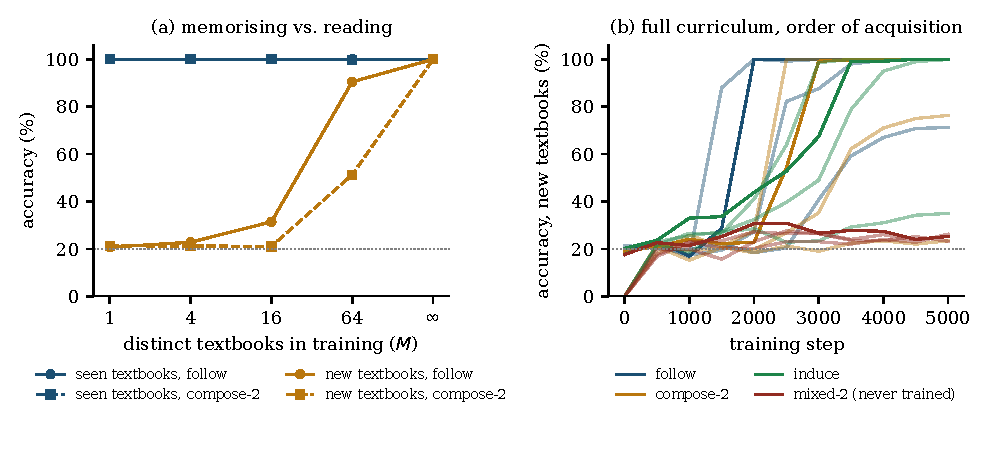
\includegraphics[width=\linewidth]{gen/fig_e1_e2.pdf}
\caption{\textbf{(a)} E1 (means over seeds). All models answer almost perfectly on their training textbooks; only those trained on enough distinct textbooks can use a new one. \textbf{(b)} E2, full curriculum, accuracy on new textbooks during training for each seed (later seeds are drawn lighter). The skills are acquired one after another in abrupt steps, and the never-trained combination \skill{mixed} stays at the guessing level. Dotted line: 20\%.}
\label{fig:e1e2}
\end{figure}

Table~\ref{tab:e1} and Figure~\ref{fig:e1e2}a show the outcome.
Every model answers exercises about its training textbooks almost perfectly.
For $M \le 16$ that is all it can do: on a new textbook, \skill{follow} accuracy is \EOneMOneNewFollow\%, \EOneMFourNewFollow\% and \EOneMOneSixNewFollow\% for $M = 1, 4, 16$.
These models have stored their textbooks in the weights and do not consult the page in front of them.
With $M = 64$ the same architecture, trained for the same number of steps, begins to use textbooks it has never seen: over two seeds it follows their rules at \EOneMSixFourNewFollowList\% and composes them at \EOneMSixFourNewComposeTwoList\%.
With an unlimited supply, both seeds reach at least \EOneMInfNewFollowMin\% on \skill{follow} and \EOneMInfNewComposeTwoMin\% on \skill{compose}.

The switch from memorising to reading as the number of distinct textbooks grows is the instructional-material counterpart of the task-diversity threshold reported for in-context regression \citep{raventos2023diversity} and for modular arithmetic \citep{he2024grok}.
Four points are worth drawing out.

\emph{Accuracy on seen material is uninformative.}
The G0 columns are the same, to within half a point, for models that read and models that do not.
Any evaluation in which the rules were available during training, in whatever form, cannot distinguish the two.

\emph{Variety made the difference, not volume.}
Every model saw the same 160{,}000 training episodes.
What changed is how many different textbooks those episodes were about.
This is the first half of hypothesis H3 in Section~\ref{sec:protocol}.

\emph{The harder skill asks for more variety.}
At $M=64$, \skill{follow} transfers to new textbooks largely or completely (\EOneMSixFourNewFollowList\%) while \skill{compose} lags behind (\EOneMSixFourNewComposeTwoList\%).
With one or two seeds per condition we do not read more into the location of the threshold than that reading begins somewhere between 16 and 64 textbooks for the easier skill and is not complete at 64 for the harder one.

\emph{Knowledge in the weights did not help with a new page.}
The models with $M \le 16$ know their textbooks perfectly and are at or near chance on a new one.
This bears on hypothesis H2 only indirectly: the direct test, adding facts to the weights of a model that already reads, is left to the full-scale study.

